%%
%% Berliner Hochschule für Technik -- Praxisphasenbericht
%%
%% Hauptdokument
%%
%% Strukturiert nach wissenschaftlichem Bachelor-Arbeit Format
%%
%%%%%%%%%%%%%%%%%%%%%%%%%%%%%%%%%%%%%%%%%%%%%%%%%%%%%%%%%%%%%%%%%%%%%

\documentclass[11pt, a4paper, oneside]{book}

%% Übersetzen für die Abgabe
\usepackage[abgabe]{resources/bht-standard/bhtThesis}
\typeout{BHT-Abschlussarbeit V2.0 26.08.21 S.Tschirley}

\usepackage{listings}
\lstset{ 
  literate={ö}{{\"o}}1
           {ä}{{\"a}}1
           {ü}{{\"u}}1
           {Ö}{{\"O}}1
           {Ä}{{\"A}}1
           {Ü}{{\"U}}1
           {ß}{{\ss}}1
}

\usepackage{siunitx}
\usepackage{bytefield}
\usepackage{hyperref}

%%
%% Pfad zu den Bildern
%%
\graphicspath{
  {pictures/},
  {graphics/}
}

%%
%% Einbinden persönlicher macros 
%%
\input{resources/src/personalMacros}

%% Message
\typeout{-----------------------------------------------------------}
\typeout{----> main.tex ---- Zentrales Dokument---------------------}
\typeout{-----------------------------------------------------------}

\version{1.0}
\datum{\today}

%%
%% Titel, Autor und Betreuer
%%
\fachbereich{VII -- Elektrotechnik -- Mechatronik -- Optometrie} 
\studiengang{Humanoide Robotik}
\autor{Tjorven Koopmann}
\edvnr{937274}
\titel{Embedded Systems Entwicklung in der industriellen Automatisierungstechnik}
\untertitel{Praxisphasenbericht über die Firmware-Entwicklung bei der ATN Automatisierungstechnik Niemeier GmbH}
\betreuerFeld{
  \begin{tabular}{lr}
    \multicolumn{2}{l}{\textbf{Gutachter}}\\
    Prof.~Dr.~Manfred Hild & Berliner Hochschule für Technik\\
    Andreas Senoner & ATN Automatisierungstechnik Niemeier\\
    Dipl.-Ing. Jörg Niemeier & ATN Automatisierungstechnik Niemeier
  \end{tabular}
}

\begin{document}
\pagestyle{fancy}

%%
%% Berliner Hochschule für Technik --  Abschlussarbeit
%%
%% Titelseiten und Erklärungen 
%%
%%%%%%%%%%%%%%%%%%%%%%%%%%%%%%%%%%%%%%%%%%%%%%%%%%%%%%%%%%%%%%%%%%%%%

\maketitle
\clearpage
%\thispagestyle{empty}
% Rueckseite (leer)
%% 
~

%%
%% Berliner Hochschule für Technik -- Praxisphasenbericht
%%
%% Kurzfassung
%%
%%%%%%%%%%%%%%%%%%%%%%%%%%%%%%%%%%%%%%%%%%%%%%%%%%%%%%%%%%%%%%%%%%%%%

\chapter*{Kurzfassung}
\addcontentsline{toc}{chapter}{Kurzfassung}

Dieser Bericht dokumentiert die Praxisphase im Zeitraum vom 07.07.2025 bis 30.11.2025 bei der Automatisierungstechnik Niemeier GmbH (ATN) in Berlin, einem Unternehmen im Bereich Automatisierungstechnik für die Elektronikfertigung. Der Schwerpunkt der Tätigkeit lag auf der Firmware-Entwicklung für Steuerungssysteme von Löt- und Dosierautomaten.

Die Arbeit folgt einer wissenschaftlichen Struktur und gliedert sich in sechs Kapitel: Nach einer Einleitung mit Problemstellung und Zielsetzung werden die theoretischen Grundlagen der Embedded-Systems-Entwicklung dargelegt. Das Methodenkapitel beschreibt die Arbeitsumgebung und angewandten Entwicklungsprozesse. Die Implementierung dokumentiert die technische Umsetzung der drei Hauptprojekte, deren Ergebnisse anschließend evaluiert werden. Das abschließende Kapitel diskutiert die Erkenntnisse und gibt einen Ausblick.

Die Praxisphase umfasste drei zentrale Tätigkeitsbereiche: Die Entwicklung eines Treibers für den TMC5160 Stepper-Motor-Controller mit präzisen Rampenprofil-Kalkulationen, die Erstellung eines Hardware-Test-Setups mittels Raspberry Pi Pico für Sensorkalibrierung, sowie das Hauptprojekt -- die vollständige Integration eines W5500 Ethernet-Controllers in die produktive Firmware.

Das Hauptprojekt erstreckte sich über 3,5 Monate und beinhaltete die Migration von einer C++-basierten Testimplementierung zu einer nativen C-Implementierung, die Entwicklung eines Compatibility-Layers für bestehende Module sowie die Implementierung fortgeschrittener Konzepte wie statisch allokierte Buffer-Pools und asynchrone SPI-Kommunikation mit freeRTOS-Context-Switching.

Zentrale Herausforderungen waren die Vermeidung von Race-Conditions in Multi-Threading-Umgebungen und die Integration neuer Komponenten in Legacy-Code ohne Beeinträchtigung bestehender Funktionalität. Die iterative Entwicklungsmethodik mit regelmäßigen Code-Reviews erwies sich als besonders geeignet für die Komplexität der Embedded-Entwicklung.

Die Praxisphase ermöglichte den Erwerb tiefgehender praktischer Kenntnisse in RTOS-Programmierung, Hardware-naher Software-Entwicklung und professionellem Projektmanagement. Die Kombination aus theoretischem Studium und praktischer Anwendung bestätigte das Interesse an Embedded Systems und legte eine solide Grundlage für die weitere berufliche Entwicklung in diesem Bereich.

\clearpage

\vspace{10ex}
\section*{Erklärung}
Ich  versichere, dass  ich diese  Abschlussarbeit ohne  fremde  Hilfe selbstständig
verfasst und  nur die  angegebenen Quellen und  Hilfsmittel benutzt  habe. Wörtlich
oder dem  Sinn nach  aus anderen  Werken entnommene Stellen  sind unter  Angabe der
Quellen kenntlich gemacht.
\vspace{10ex}\\

\hrule
{\small{Datum}}\hfill{\small{Unterschrift}}


\pagenumbering{roman}
\tableofcontents
\listoffigures




\pagenumbering{arabic}
%%%%%%%%%%%%%%%%%%%%%%%%%%%%%%%%%%%%%%%%%%%%%%%%%%%%%%%%%%%%%%%
%% Die Kapitel der Arbeit -- Wissenschaftliche Struktur
\newpage
\chapter{Einleitung}
\label{chap:einleitung}

\section{Motivation und Problemstellung}
\label{sec:motivation}

% TODO: Persönliche Motivation konkretisieren - warum genau ATN? Wie auf die Stelle aufmerksam geworden?

Die Entwicklung von Embedded Systems für industrielle Automatisierungsanwendungen stellt eine der zentralen Herausforderungen der modernen Fertigungstechnik dar. Die zunehmende Komplexität von Steuerungssystemen erfordert eine enge Verzahnung von Hardware-naher Programmierung, Echtzeitsystemen und Netzwerkkommunikation. Diese Arbeit dokumentiert die praktische Anwendung theoretischer Studieninhalte im Bereich der Firmware-Entwicklung während einer Praxisphase bei der Automatisierungstechnik Niemeier GmbH (ATN) in Berlin.

% TODO: Weg zur Praxisstelle beschreiben (Bewerbungsprozess, erste Kontakte, etc.)

Die Entscheidung für diese Praxisstelle basierte auf dem starken Interesse an Embedded Systems und Firmware-Entwicklung. Während des Studiums der Humanoiden Robotik wurden in mehreren Modulen Grundlagen der Mikrocontroller-Programmierung und hardwarenahen Entwicklung vermittelt. Die praktischen Übungen im Bereich der hardwarenahen Programmierung zeigten, dass die Verbindung zwischen Software und Hardware genau der Bereich ist, in dem eine Vertiefung angestrebt wurde.

\section{Zielsetzung der Arbeit}
\label{sec:zielsetzung}

Das übergeordnete Ziel dieser Praxisphase war die Entwicklung produktionsreifer Firmware-Komponenten für industrielle Automatisierungssysteme. Im Einzelnen wurden folgende Teilziele definiert:

\begin{enumerate}
    \item \textbf{TMC5160 Stepper-Motor-Driver:} Entwicklung präziser Rampenprofil-Kalkulationen für einen Lötvorschub-Modul unter Berücksichtigung von Interrupt-Sicherheit und Echtzeitanforderungen.
    
    \item \textbf{Hardware-Testing:} Entwicklung eines kostengünstigen Prototyping-Systems zur Sensorkalibrierung mittels Raspberry Pi Pico als USB-Host.
    
    \item \textbf{W5500 Ethernet-Integration:} Vollständige Integration eines Ethernet-Controllers in die bestehende Firmware-Architektur mit Fokus auf asynchrone Kommunikation und statisches Speichermanagement.
\end{enumerate}

Die Arbeit verfolgt dabei einen wissenschaftlich-methodischen Ansatz, der die Verknüpfung zwischen theoretischem Studienwissen und praktischer Anwendung explizit dokumentiert.

\section{Aufbau der Arbeit}
\label{sec:aufbau}

Die vorliegende Arbeit gliedert sich in sechs Kapitel, die einer wissenschaftlichen Struktur folgen:

\textbf{Kapitel~\ref{chap:grundlagen}} legt die theoretischen Grundlagen der Embedded-Systems-Entwicklung dar. Es werden die relevanten Konzepte aus dem Studium -- insbesondere Echtzeitbetriebssysteme, Speicherverwaltung und Hardware-Kommunikation -- erläutert und in den Kontext der industriellen Automatisierungstechnik eingeordnet.

\textbf{Kapitel~\ref{chap:methodik}} beschreibt die Arbeitsumgebung und die angewandten Methoden. Neben der Vorstellung des Praktikumsbetriebs werden die verwendeten Entwicklungswerkzeuge, Prozesse und die organisatorischen Rahmenbedingungen dargestellt.

\textbf{Kapitel~\ref{chap:implementierung}} dokumentiert die technische Implementierung der drei Hauptprojekte. Der Schwerpunkt liegt auf der detaillierten Beschreibung der Lösungsansätze und deren technischer Umsetzung.

\textbf{Kapitel~\ref{chap:ergebnisse}} präsentiert die erzielten Ergebnisse und evaluiert deren Qualität anhand definierter Kriterien. Die Projektergebnisse werden sowohl quantitativ als auch qualitativ bewertet.

\textbf{Kapitel~\ref{chap:diskussion}} diskutiert die gewonnenen Erkenntnisse im Kontext des Studiums und der beruflichen Entwicklung. Es werden Verbesserungspotenziale identifiziert und ein Ausblick auf zukünftige Entwicklungen gegeben.

\section{Abgrenzung}
\label{sec:abgrenzung}

Diese Arbeit fokussiert sich auf die Firmware-Entwicklung für Embedded Systems im Kontext der industriellen Automatisierungstechnik. Nicht behandelt werden:

\begin{itemize}
    \item Hardware-Design und Schaltungsentwicklung
    \item Mechanische Konstruktion (außer unterstützende CAD-Arbeiten)
    \item Vertriebliche oder kaufmännische Aspekte
    \item Zertifizierungs- und Zulassungsverfahren
\end{itemize}

Der zeitliche Rahmen der Praxisphase erstreckte sich vom 07.07.2025 bis 30.11.2025, wobei krankheitsbedingte Unterbrechungen zwischen dem 15.09. und 01.11. zu verzeichnen waren.
           % Kapitel 1: Einleitung
\chapter{Theoretische Grundlagen}
\label{chap:grundlagen}

Dieses Kapitel legt die theoretischen Grundlagen dar, die für das Verständnis der durchgeführten Arbeiten erforderlich sind.

\section{Embedded Systems und Firmware-Entwicklung}
\label{sec:embedded_systems}

Embedded Systems sind spezialisierte Computersysteme, die als Teil eines größeren Systems dedizierte Funktionen ausführen. Im Gegensatz zu General-Purpose-Computern sind sie für spezifische Aufgaben optimiert und unterliegen strengen Anforderungen bezüglich Ressourcenverbrauch, Echtzeitfähigkeit und Zuverlässigkeit.

\subsection{Charakteristiken von Embedded Systems}

Die grundlegenden Charakteristiken von Embedded Systems umfassen:

\begin{itemize}
    \item \textbf{Ressourcenbeschränkungen:} Limitierter Speicher, Rechenleistung und Energieverbrauch
    \item \textbf{Echtzeitanforderungen:} Deterministische Reaktionszeiten auf externe Ereignisse
    \item \textbf{Hardware-Nähe:} Direkte Interaktion mit Peripherie über Register und Interrupts
    \item \textbf{Zuverlässigkeit:} Langzeitstabilität ohne menschliche Intervention
\end{itemize}

Diese Charakteristiken haben direkte Auswirkungen auf die Softwarearchitektur und die verwendeten Programmiertechniken.

\subsection{C versus C++ in Embedded-Kontexten}

Die Wahl der Programmiersprache in Embedded Systems ist eine wichtige Architekturentscheidung. Während C++ mit seinen objektorientierten Konzepten Vorteile in der Strukturierung bietet, führt es zu zusätzlichem Overhead:

\begin{itemize}
    \item Virtuelle Funktionstabellen erhöhen Speicherverbrauch
    \item Runtime Type Information (RTTI) benötigt zusätzliche Ressourcen
    \item Exceptions können zu nicht-deterministischem Verhalten führen
\end{itemize}

Native C bietet hingegen maximale Kontrolle über den generierten Maschinencode und minimalen Overhead. Die Entscheidung zwischen beiden Sprachen muss projektspezifisch getroffen werden.

\section{Echtzeitbetriebssysteme (RTOS)}
\label{sec:rtos}

Ein Echtzeitbetriebssystem (Real-Time Operating System, RTOS) ist ein Betriebssystem, das deterministische Reaktionszeiten garantiert.

\subsection{Scheduling und Task-Management}

Das Scheduling in einem RTOS folgt in der Regel einem prioritätsbasierten präemptiven Ansatz. Jeder Task erhält eine Priorität, und der Scheduler wählt stets den bereiten Task mit der höchsten Priorität zur Ausführung.

\nlparagraph{Task-Zustände}
Ein Task kann sich in folgenden Zuständen befinden:
\begin{itemize}
    \item \textbf{Running:} Aktuell in Ausführung
    \item \textbf{Ready:} Bereit zur Ausführung, wartet auf Scheduler
    \item \textbf{Blocked:} Wartet auf ein Ereignis (z.B. Semaphor, Timer)
    \item \textbf{Suspended:} Explizit angehalten
\end{itemize}

\subsection{Synchronisationsmechanismen}

Die Koordination zwischen Tasks erfordert Synchronisationsmechanismen:

\nlparagraph{Semaphoren}
Semaphoren sind Zählvariablen, die den Zugriff auf begrenzte Ressourcen kontrollieren. Binäre Semaphoren (Werte 0 oder 1) dienen der Signalisierung zwischen Tasks.

\nlparagraph{Mutexe}
Mutexe (Mutual Exclusion) schützen kritische Abschnitte vor gleichzeitigem Zugriff. Im Gegensatz zu Semaphoren implementieren sie das Ownership-Konzept und können Priority Inheritance unterstützen.

\nlparagraph{Message Queues}
Message Queues ermöglichen asynchrone Kommunikation zwischen Tasks durch das Senden und Empfangen von Nachrichten. Sie entkoppeln Sender und Empfänger zeitlich.

\subsection{Interrupt Service Routines (ISR)}
\label{subsec:isr}

Interrupts ermöglichen die sofortige Reaktion auf Hardware-Ereignisse. Die Interrupt Service Routine (ISR) ist dabei eine spezielle Funktion, die außerhalb des normalen Task-Kontexts ausgeführt wird.

\nlparagraph{ISR-Kontext vs. Task-Kontext}
Der ISR-Kontext unterscheidet sich fundamental vom Task-Kontext:
\begin{itemize}
    \item ISRs dürfen nicht blockieren
    \item Viele RTOS-Funktionen sind im ISR-Kontext nicht verfügbar
    \item ISRs sollten möglichst kurz sein
    \item Die Kommunikation mit Tasks erfolgt über spezielle ISR-sichere Mechanismen
\end{itemize}

\section{Speicherverwaltung in Embedded Systems}
\label{sec:speicherverwaltung}

Die Speicherverwaltung in Embedded Systems unterscheidet sich grundlegend von der in Desktop-Systemen.

\subsection{Statische vs. Dynamische Allokation}

\nlparagraph{Dynamische Allokation}
Dynamische Speicherallokation mittels \texttt{malloc()} und \texttt{free()} ist in Embedded Systems problematisch:
\begin{itemize}
    \item \textbf{Fragmentierung:} Wiederholte Allokation/Deallokation führt zu Speicherfragmentierung
    \item \textbf{Nicht-deterministisch:} Die Ausführungszeit von \texttt{malloc()} ist nicht vorhersagbar
    \item \textbf{Fehlerbehandlung:} Out-of-Memory-Situationen zur Laufzeit sind schwer handhabbar
\end{itemize}

\nlparagraph{Statische Allokation}
In sicherheitskritischen und echtzeitfähigen Systemen wird daher oft statische Allokation bevorzugt:
\begin{itemize}
    \item Speicher wird zur Compile-Zeit reserviert
    \item Deterministische Laufzeit
    \item Keine Fragmentierung möglich
    \item Ressourcenverbrauch ist zur Entwicklungszeit bekannt
\end{itemize}

\subsection{Buffer-Pool-Konzept}

Das Buffer-Pool-Konzept verbindet die Vorteile beider Ansätze: Statisch allozierte Buffer werden zur Laufzeit aus einem Pool angefordert und nach Gebrauch zurückgegeben. Dies ermöglicht flexible Ressourcennutzung bei deterministischem Verhalten.

\section{Hardware-Kommunikation}
\label{sec:hardware_kommunikation}

Die Kommunikation mit Hardware-Komponenten erfolgt über verschiedene Protokolle und Schnittstellen.

\subsection{Serial Peripheral Interface (SPI)}

SPI ist ein synchrones serielles Kommunikationsprotokoll für die Kommunikation zwischen Mikrocontrollern und Peripheriegeräten. Es verwendet vier Signalleitungen:

\begin{itemize}
    \item \textbf{SCLK:} Serial Clock (vom Master generiert)
    \item \textbf{MOSI:} Master Out Slave In
    \item \textbf{MISO:} Master In Slave Out
    \item \textbf{CS:} Chip Select (aktiv low)
\end{itemize}

SPI ermöglicht hohe Datenraten und Vollduplex-Kommunikation, erfordert jedoch für jeden Slave eine separate Chip-Select-Leitung.

\subsection{TCP/IP und Ethernet}

Das TCP/IP-Protokollstack ermöglicht die Kommunikation über Ethernet-Netzwerke. Die relevanten Schichten für Embedded-Anwendungen sind:

\begin{itemize}
    \item \textbf{Physical/Data Link:} Ethernet (IEEE 802.3)
    \item \textbf{Network:} Internet Protocol (IP)
    \item \textbf{Transport:} Transmission Control Protocol (TCP) / User Datagram Protocol (UDP)
    \item \textbf{Application:} Anwendungsspezifische Protokolle
\end{itemize}

Hardware-TCP/IP-Stacks wie der W5500 implementieren diese Schichten in Hardware und entlasten damit den Hauptprozessor.

\section{Schrittmotorsteuerung}
\label{sec:schrittmotorsteuerung}

Schrittmotoren sind Synchronmotoren, die durch diskrete Spannungspulse angesteuert werden. Für präzise Bewegungen sind geeignete Rampenprofile erforderlich.

\subsection{Rampenprofile}

Ein Rampenprofil beschreibt den zeitlichen Verlauf der Geschwindigkeit während einer Bewegung. Typische Profile umfassen:

\begin{itemize}
    \item \textbf{Beschleunigungsphase:} Lineare Erhöhung der Geschwindigkeit
    \item \textbf{Konstantfahrt:} Bewegung mit Maximalgeschwindigkeit
    \item \textbf{Verzögerungsphase:} Lineare Reduktion der Geschwindigkeit
\end{itemize}

Die mathematische Modellierung dieser Phasen erfordert die Berechnung von Beschleunigung, Zeit und zurückgelegter Strecke unter Berücksichtigung physikalischer Constraints des Motors.
           % Kapitel 2: Theoretische Grundlagen
\chapter{Methodik und Arbeitsumgebung}
\label{chap:methodik}

Dieses Kapitel beschreibt die Arbeitsumgebung, in der die Praxisphase durchgeführt wurde, sowie die angewandten Methoden und Prozesse. Eine fundierte Darstellung dieser Rahmenbedingungen ist für die Einordnung der technischen Ergebnisse unerlässlich.

\section{Vorstellung des Praktikumsbetriebs}
\label{sec:praktikumsbetrieb}

\subsection{Unternehmensprofil}

% TODO: Foto des Firmengebäudes oder Arbeitsplatzes einfügen?

Die Automatisierungstechnik Niemeier GmbH (ATN) mit Standort in Berlin-Treptow-Köpenick entwickelt, produziert und vertreibt Komponenten, Systeme und Software für die Elektronikfertigung. Die Kernkompetenzen umfassen Löttechnik, Lötroboter, Dosiertechnik und Maschinen für die SMT-Fertigung.

Das Unternehmen wurde 1996 als Ausgründung aus dem Produktionstechnischen Zentrum Berlin (PTZ) der TU Berlin gegründet und beschäftigt aktuell etwa 40 Mitarbeiter. Die universitären Wurzeln spiegeln sich in der engen Kooperation mit Hochschulen und Forschungsinstituten wider.

\subsection{Marktposition und Produkte}

% TODO: Produktfotos einfügen (LightBeam-System, VARIO-Plattform, Lötsystem)?

ATN hat sich in mehreren Marktsegmenten als Spezialist positioniert:

\nlparagraph{Selektives Lichtlöten}
Mit dem LightBeam-System hat sich ATN als Marktführer für selektives Lichtlöten in der Elektronikfertigung etabliert. Das modulare Lötsystem VARIO bietet eine flexible Plattform für verschiedene Löttechnologien.

\nlparagraph{Solarmodulfertigung}
Mit über 300 weltweit installierten Induktionslötsystemen gehört ATN zu den Marktführern für das automatisierte Löten der Randverschaltung von Solarmodulen.

\nlparagraph{Dosiertechnik}
Als autorisierter Vertriebs- und Service-Partner von Musashi Engineering bedient ATN Kunden in der optoelektronischen Industrie und Medizintechnik.

\subsection{Organisationsstruktur}

% TODO: Organigramm oder vereinfachte Darstellung der Unternehmensstruktur?

Die Organisationsstruktur von ATN umfasst folgende Bereiche:
\begin{itemize}
    \item Applikation Löten
    \item Konstruktion
    \item Steuerungsentwicklung und -bau
    \item Programmierung
    \item Vertrieb und Service
\end{itemize}

Die Praxisphase wurde im Bereich Steuerungsentwicklung und Programmierung durchgeführt, konkret im Elektronik-Labor.

\section{Arbeitsumgebung und Ressourcen}
\label{sec:arbeitsumgebung}

\subsection{Technische Infrastruktur}

Für die Firmware-Entwicklung standen professionelle Entwicklungswerkzeuge zur Verfügung:

\nlparagraph{Entwicklungsumgebung}
\begin{itemize}
    \item IDE für Embedded-Entwicklung (proprietäre Toolchain)
    \item Versionskontrolle (Git)
    \item Debugging-Tools (JTAG/SWD-Debugger)
    \item Logic-Analyzer für Signalanalyse
\end{itemize}

\nlparagraph{Hardware}
\begin{itemize}
    \item TMC5160 Stepper-Motor-Controller (Evaluationsboards und Eigenentwicklung)
    \item W5500 Ethernet-Controller (Evaluationsmodul und Addon-Board)
    \item Raspberry Pi Pico für Prototyping
    \item 3D-Drucker für mechanisches Prototyping
\end{itemize}

\subsection{Firmware-Architektur (ATNC3)}

Die interne ATN-Control-3-Firmware (ATNC3) stellt die Basis für alle Steuerungssysteme dar. Die Architektur basiert auf freeRTOS und implementiert:

\begin{itemize}
    \item Modulares Task-System mit definierten Schnittstellen
    \item Bus-Device-Handler für Hardware-Abstraktion
    \item SPI-Task-Struktur mit Queue-basierter Kommunikation
    \item Integrierte User-Interface-Komponenten
\end{itemize}

Die Integration neuer Komponenten erfordert die Einhaltung dieser Architekturvorgaben.

\section{Betreuung und Zusammenarbeit}
\label{sec:betreuung}

\subsection{Fachliche Ansprechpartner}

Die direkte fachliche Betreuung erfolgte durch:
\begin{itemize}
    \item \textbf{Thomas Wolf:} Erfahrener Firmware-Entwickler, Hauptansprechpartner für Architektur und Code-Reviews
    \item \textbf{Pascal Rosin:} Firmware-Entwickler, Unterstützung bei freeRTOS-spezifischen Themen
\end{itemize}

\subsection{Arbeitsorganisation}

Die Arbeitsorganisation folgte einem strukturierten Prozess:
\begin{itemize}
    \item Wöchentliche Abstimmungen zu Projektfortschritt und Priorisierung
    \item Regelmäßige Code-Reviews vor Integration in die Hauptcodebasis
    \item Dokumentation von Entscheidungen und technischen Lösungen
    \item Eigenverantwortliche Zeiteinteilung bei definierten Meilensteinen
\end{itemize}

\section{Angewandte Methoden}
\label{sec:methoden}

\subsection{Entwicklungsprozess}

Der Entwicklungsprozess orientierte sich an iterativen Methoden:

\nlparagraph{Iterative Entwicklung}
Komplexe Funktionalitäten wurden in Iterationen entwickelt:
\begin{enumerate}
    \item Analyse und Konzeption
    \item Implementierung eines funktionalen Prototyps
    \item Integration und Testing
    \item Review und Refactoring
    \item Dokumentation
\end{enumerate}

\nlparagraph{Code-Reviews}
Code-Reviews waren integraler Bestandteil des Entwicklungsprozesses. Sie dienten:
\begin{itemize}
    \item Der Qualitätssicherung
    \item Dem Wissenstransfer
    \item Der Einhaltung von Coding-Standards
    \item Der frühzeitigen Identifikation von Architekturproblemen
\end{itemize}

\subsection{Testing-Strategien}

\nlparagraph{Hardware-in-the-Loop}
Aufgrund der Hardware-Abhängigkeit der Firmware erfolgte das Testing primär auf echter Hardware. Systematisches Logging ermöglichte die Nachverfolgung von Problemen.

\nlparagraph{Stress-Testing}
Kritische Komponenten wurden unter erhöhter Last getestet, um Race-Conditions und Timing-Probleme zu identifizieren.

\subsection{Dokumentation}

Die Dokumentation umfasste:
\begin{itemize}
    \item Code-Kommentare gemäß internem Standard
    \item Technische Dokumentation von Schnittstellen
    \item Commit-Messages mit Beschreibung der Änderungen
    \item Notizen zu Design-Entscheidungen
\end{itemize}

\section{Mitgebrachte Qualifikationen}
\label{sec:qualifikationen}

Folgende Vorkenntnisse waren für die Praxisphase relevant:

\nlparagraph{Programmierkenntnisse}
\begin{itemize}
    \item Kenntnisse in C und C++
    \item Verständnis von Pointern und Speicherverwaltung
    \item Erfahrung mit Versionskontrolle (Git)
    \item Debugging-Grundlagen
\end{itemize}

\nlparagraph{Embedded Systems}
\begin{itemize}
    \item Grundwissen über Mikrocontroller-Architekturen
    \item Theoretische Kenntnisse in RTOS-Konzepten
    \item Verständnis für Hardware-Software-Schnittstellen
\end{itemize}

\nlparagraph{CAD und Prototyping}
\begin{itemize}
    \item Erfahrung mit SolidWorks
    \item Grundkenntnisse im 3D-Druck
\end{itemize}

Diese Vorkenntnisse bildeten eine solide Basis, auch wenn viele Aspekte der professionellen Embedded-Entwicklung während der Praxisphase neu erlernt werden mussten.

\section{Projektübersicht}
\label{sec:projektuebersicht}

Die Praxisphase umfasste drei Hauptprojekte, die in Kapitel~\ref{chap:implementierung} detailliert beschrieben werden:

\begin{enumerate}
    \item \textbf{TMC5160 Stepper-Motor-Driver} (ca. 4 Wochen): Implementierung der Rampenprofil-Kalkulationen für einen Lötvorschub-Modul
    
    \item \textbf{Hardware-Testing-System} (ca. 1 Woche): Entwicklung eines USB-Host-Systems zur Sensorkalibrierung
    
    \item \textbf{W5500 Ethernet-Integration} (ca. 14 Wochen): Vollständige Integration eines Ethernet-Controllers in die produktive Firmware
\end{enumerate}

Die Projekte waren aufeinander aufbauend konzipiert: Die Erfahrungen aus den ersten beiden Projekten -- insbesondere im Umgang mit der ATNC3-Firmware und freeRTOS -- bildeten die Grundlage für das umfangreiche Hauptprojekt.
             % Kapitel 3: Methodik und Arbeitsumgebung
\chapter{Implementierung}
\label{chap:implementierung}

Dieses Kapitel dokumentiert die technische Implementierung der drei Hauptprojekte. Der Fokus liegt auf der detaillierten Beschreibung der Lösungsansätze, der aufgetretenen Herausforderungen und deren Bewältigung.

\section{TMC5160 Stepper-Motor-Driver}
\label{sec:tmc5160}

\subsection{Aufgabenstellung und technischer Hintergrund}

% TODO: Foto oder Schaltbild des Lötvorschub-Moduls einfügen?

Das erste Projekt konzentrierte sich auf die Mitentwicklung eines Lötvorschub-Moduls basierend auf dem TMC5160 Stepper-Motor-Controller von Trinamic. Das Modul wurde in C++ geschrieben und mittels C-Wrapper in die ATNC3-Firmware eingebunden.

Der Aufgabenbereich umfasste die Implementierung der Runtime-Berechnungen des Rampenprofils (Abbildung~\ref{fig:tmc_rampenprofil}).

\begin{figure}[h]
\centering
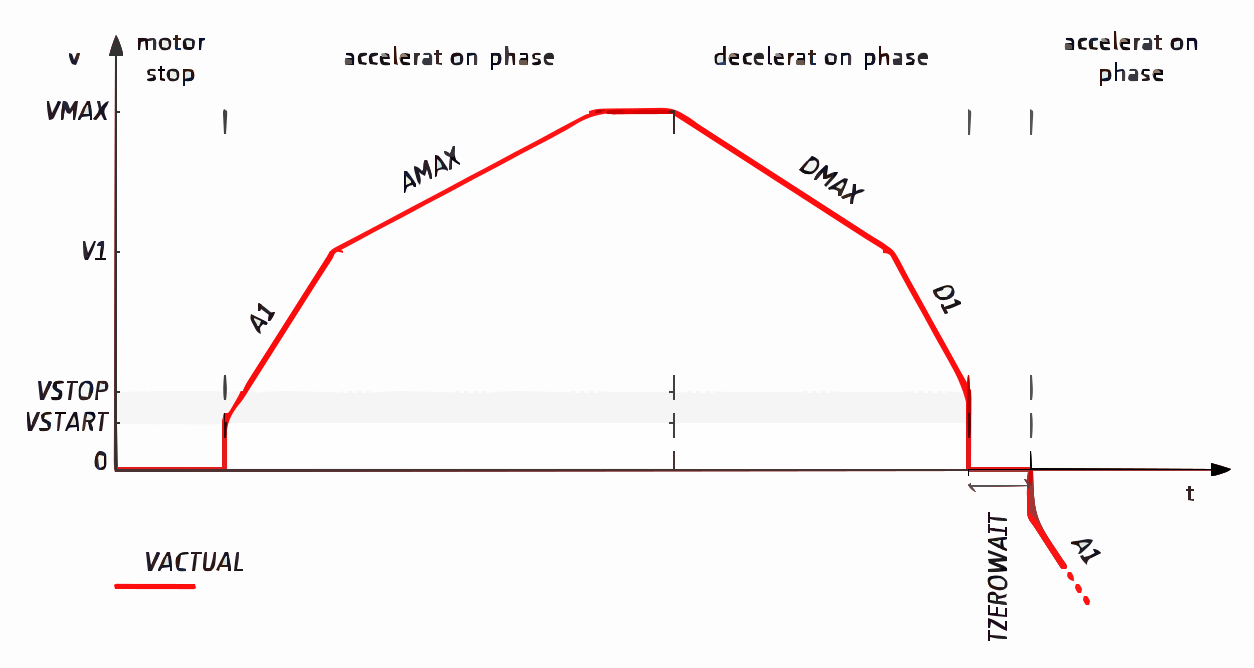
\includegraphics[scale=.6]{chapters/4_implementierung/graphics/tmc_ramp_profile.png}
\caption{TMC5160 Rampenprofil}
\label{fig:tmc_rampenprofil}
\end{figure}

\subsection{Mathematische Modellierung}

Das Rampenprofil wurde in fünf charakteristische Teilsektionen unterteilt (Abbildung~\ref{fig:tmc_rampenprofil_split}).

\begin{figure}[h]
\centering
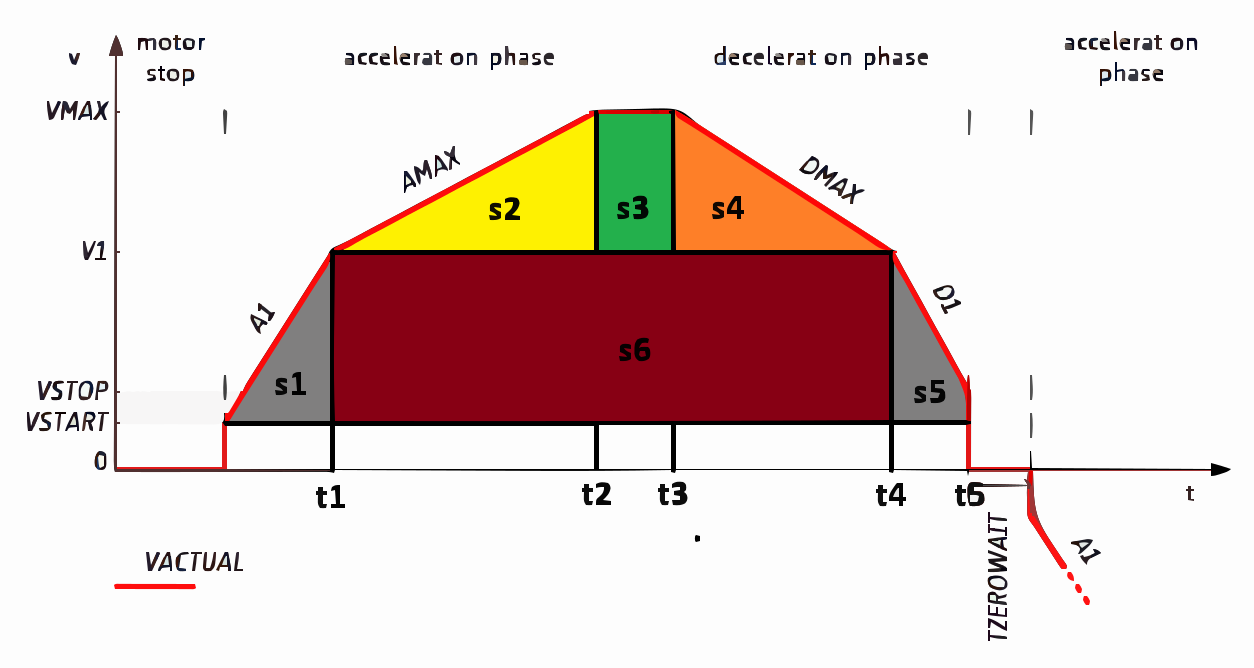
\includegraphics[scale=.6]{chapters/4_implementierung/graphics/tmc_ramp_profile_split.png}
\caption{Aufgeteiltes TMC5160 Rampenprofil mit Sektionen}
\label{fig:tmc_rampenprofil_split}
\end{figure}

\nlparagraph{Eingabeparameter}
Die benutzerdefinierten Eingabeparameter sind in Tabelle~\ref{tab:tmc5160_rampprofile_parameters} dargestellt.

\begin{table}[ht]
    \centering
    \begin{tabular}{c|c|l}
         Parameter & Einheit & Beschreibung \\ 
         \hline
         $V_{feed}$ & \unit{\frac{steps}{s}} & Vorschubgeschwindigkeit \\
         $V_1$ & \unit{\frac{steps}{s}} & Zwischengeschwindigkeit \\
         $t_{feed}$ & \unit{s} & Gesamtzeit \\
         $f_{accel}$ & \unit{\%} & Beschleunigungsfaktor \\
         $f_{decel}$ & \unit{\%} & Verzögerungsfaktor \\
    \end{tabular}
    \caption{Rampenprofil Eingabeparameter}
    \label{tab:tmc5160_rampprofile_parameters}
\end{table}

\nlparagraph{Randbedingungen}
Die Berechnungen erfolgen unter folgenden Randbedingungen:
\[V_{Stop} = V_{Start} = 0\]
\[t_{feed_{min}} = 0.1 < t_{feed} \]
\[S_{total} = V_{feed} \cdot t_{feed} = s_1 + s_2 + s_3 + s_4 + s_5\]

\nlparagraph{Berechnung von $V_{max}$}
Die maximale Geschwindigkeit wird wie folgt berechnet:
\[\mu_1 = 2 \cdot t_{feed_{min}} + \frac{(t_{feed} - 2 \cdot t_{feed_{min}}) \cdot (f_{accel} + f_{decel})}{2}\]
\[\mu_2 = (t_{feed} - 2 \cdot t_{feed_{min}}) \cdot (1 - \frac{f_{accel}}{2} - \frac{f_{decel}}{2})\]
\[V_{max} = \frac{V_{feed} \cdot t_{feed} - V_1 \cdot \mu_1}{\mu_2}\]

\nlparagraph{Rampenparameter}
Die Beschleunigungs- und Verzögerungswerte werden wie folgt modelliert:
\[A_1 = \frac{V_1}{t_1}, \quad A_{max} = \frac{V_{max} - V_1}{t_2}\]
\[D_1 = \frac{V_1}{-t_5}, \quad D_{max} = \frac{V_1 - V_{max}}{t_4}\]

\subsection{Programmatische Implementierung}

Die Implementierung erfolgte als Teil der \texttt{sf\_stepper}-Klasse. Die Funktion gliedert sich in mehrere Phasen:

\nlparagraph{Eingabevalidierung}
Zunächst erfolgt eine Validierung der Eingabeparameter zur Vermeidung ungültiger Berechnungen.
\lstinputlisting[caption=Eingabeparameter-Validierung, label={lst:input_validation}, language=C++]{chapters/4_implementierung/code/input_validation.c}

\nlparagraph{Berechnung}
Nach erfolgreicher Validierung werden die Einheiten konvertiert und $V_{max}$ berechnet.
\lstinputlisting[caption=Unit-Konversion und $V_{max}$-Berechnung, label={lst:vmax_calculation}, language=C++]{chapters/4_implementierung/code/vmax_calculation.c}

\nlparagraph{Konsistenzprüfung}
Abschließend erfolgt eine Plausibilitätsprüfung der Berechnungen mit definierten Toleranzen (zeitlich: 3ms, räumlich: 1 Fullstep $\approx$ 109µm).
\lstinputlisting[caption=Validierung der Berechnungen, label={lst:calculation_validation}, language=C++]{chapters/4_implementierung/code/calculation_validation.c}

\section{Hardware-Testing und Prototyping}
\label{sec:hardware_testing}

\subsection{Aufgabenstellung}

Zur Validierung des in Abschnitt~\ref{sec:tmc5160} beschriebenen TMC5160-basierten Lötvorschub-Moduls wurde ein Messsystem zur Erfassung von Bewegungsdaten benötigt. Ziel war es, die berechneten Rampenprofile mit den tatsächlichen Bewegungen des Motors zu vergleichen. Die Anforderungen waren:
\begin{itemize}
    \item Erfassung von Positionsdaten zur Verifikation der Rampenprofile
    \item Bidirektionale Messung (X/Y-Achse)
    \item Kostengünstige und zeitnahe Umsetzung (6 Tage)
\end{itemize}

Als Lösung wurde ein optischer Maussensor gewählt, der über einen Raspberry Pi Pico als USB-Host ausgelesen wird.

\subsection{Technische Realisierung}

\nlparagraph{USB-Host-Implementierung}
Der Raspberry Pi Pico wurde mittels TinyUSB-Stack und Pico PIO USB als USB-Host konfiguriert. Die PIO (Programmable I/O) des RP2040-Mikrocontrollers ermöglichte die USB-Kommunikation ohne dedizierte USB-Host-Hardware.

Die Implementierung umfasste:
\begin{itemize}
    \item Parsing des USB-HID-Protokolls
    \item Konfiguration der USB-Descriptors
    \item Interrupt-basierter Datentransfer
    \item Serielle Datenausgabe via UART
\end{itemize}

\nlparagraph{Mechanische Integration}

% TODO: Foto des Prototyps mit Maussensor und 3D-gedruckter Halterung einfügen?
% TODO: CAD-Screenshot der Halterung einfügen?

Für die Integration wurde eine Halterung mittels SolidWorks konstruiert und per FDM-3D-Druck gefertigt. Die Konstruktion berücksichtigte Sensor-Positionierung, mechanische Entkopplung und Fertigungsrestriktionen des FDM-Verfahrens.

\subsection{Evaluierung}

Die Implementierung der USB-Host-Funktionalität verlief erfolgreich. Bei der praktischen Evaluierung zur Verifikation der TMC5160-Rampenprofile zeigten sich jedoch kritische Einschränkungen des gewählten Sensorprinzips:

\begin{itemize}
    \item \textbf{Unzureichende Messgenauigkeit:} Die Abhängigkeit optischer Maussensoren von der Oberflächenbeschaffenheit führte zu inkonsistenten Messergebnissen (>5\% Fehler)
    \item \textbf{Sporadischer Tracking-Verlust:} Bei höheren Geschwindigkeiten oder inhomogenen Oberflächen gingen Messdaten verloren
    \item \textbf{Fehlende Reproduzierbarkeit:} Die Kalibrierungen zeigten hohe Streuung zwischen einzelnen Durchläufen
\end{itemize}

Durch diese Limitierungen waren die Testergebnisse für die Validierung der Lötvorschub-Rampenprofile unzuverlässig. Eine belastbare Aussage über die Korrektheit der TMC5160-Implementierung war mit diesem Messaufbau nicht möglich.

\subsection{Fazit}

Der Prototyp demonstrierte die technische Machbarkeit der USB-Host-Implementierung auf dem RP2040. Der gewählte Sensor-Typ erwies sich jedoch als ungeeignet für die geforderten Genauigkeitsanforderungen bei der Verifikation von Motorbewegungen.

Die gewonnenen Erkenntnisse führten zur Identifikation alternativer Ansätze für zukünftige Tests:
\begin{itemize}
    \item Lineare Encoder mit absoluter Positionserfassung
    \item Laser-basierte Distanzmesssysteme
    \item Inkrementalgeber mit höherer Auflösung
\end{itemize}

Trotz des negativen Evaluierungsergebnisses war die Entwicklungszeit von 6 Tagen akzeptabel, da der Rapid-Prototyping-Ansatz frühzeitig die technischen Grenzen des gewählten Sensorprinzips aufzeigte.

\section{W5500 Ethernet-Driver Integration}
\label{sec:w5500}

% TODO: Foto des W5500 Addon-Boards einfügen?
% TODO: Architekturdiagramm der Integration (SPI-Task, Buffer-Pool, etc.) erstellen?

Das Hauptprojekt der Praxisphase erstreckte sich über 3,5 Monate (08.08.2025 -- 24.11.2025) und umfasste die vollständige Integration eines W5500 Ethernet-Controllers in die ATNC3-Firmware. Zentrale Eigenentwicklung war dabei die Konvertierung des originalen WIZnet-Treibers von C zu C++ mit erweiterter Funktionalität.

\subsection{Projektphasen}

Das Projekt durchlief mehrere iterative Entwicklungsphasen:

\nlparagraph{Phase 1: Analyse und initiale Implementierung (Woche 1--3)}
\begin{itemize}
    \item Einarbeitung in Hardware-Dokumentation und W5500-Funktionsweise
    \item Entwicklung einer C++-basierten Testimplementierung
    \item Meilenstein: Funktionierende Grundkommunikation über Ethernet
\end{itemize}

\nlparagraph{Phase 2: Migration zu nativer C-Implementierung (Woche 4--6)}
\begin{itemize}
    \item Wechsel von C++ zu nativem C für Produktionsfirmware
    \item Wechsel von Evaluationsmodul zu eigenem Addon-Board
    \item Hardware-Registrierung im Bus-Device-Handler
    \item Meilenstein: Separat funktionierende C-Version
\end{itemize}

\nlparagraph{Phase 3: Firmware-Integration (Woche 7--9)}
\begin{itemize}
    \item Definition des genauen Projektumfangs
    \item Verlagerung SPI-abhängiger Funktionen in den SPI-Task
    \item Registrierung im Bus-Device-Handler
\end{itemize}

\nlparagraph{Phase 4: Interface-Entwicklung (Woche 10--12)}
\begin{itemize}
    \item Entwicklung des Ethernet-Interfaces
    \item Meilenstein: Driver integriert mit Interface für andere Module
\end{itemize}

\nlparagraph{Phase 5: Erweiterte Funktionalität (Woche 13--15)}
\begin{itemize}
    \item Implementierung statischer Buffer-Pools
    \item Implementierung asynchroner Read/Write-Funktionen
    \item Meilenstein: Produktionsreife Implementierung
\end{itemize}

\subsection{C++ Driver-Architektur}

Die C++-Testimplementierung bildete die Grundlage für das Verständnis des W5500 und diente als Referenz für die spätere C-Portierung. Der Driver wurde als objektorientierte Klassenhierarchie konzipiert, die Mehrfachvererbung nutzt.

\subsubsection{Klassenstruktur und Vererbung}

Die \texttt{W5500}-Klasse erbt von zwei Basisklassen mittels \texttt{protected} und \texttt{public} Vererbung:

\lstinputlisting[caption=W5500-Klassendeklaration mit Mehrfachvererbung, label={lst:w5500_class}, language=C++]{chapters/4_implementierung/code/w5500/w5500_class_declaration.cpp}

Diese Architektur ermöglicht:
\begin{itemize}
    \item \textbf{SPIDevice (protected):} Kapselung der SPI-Kommunikation, nicht direkt von außen zugreifbar
    \item \textbf{GPIO\_EXTI\_Handler (public):} Interrupt-Behandlung für eingehende Daten
\end{itemize}

\subsubsection{SPI-Abstraktionsschicht}

Die Basisklasse \texttt{SPIDevice} abstrahiert die hardwarenahe SPI-Kommunikation und verwaltet Chip-Select, DMA-Handles und Taktfrequenzen:

\lstinputlisting[caption=SPIDevice-Basisklasse, label={lst:spi_device}, language=C++]{chapters/4_implementierung/code/w5500/spi_device_class.cpp}

Die dynamische Baudrate-Konfiguration berechnet den optimalen Prescaler basierend auf der Peripheral-Clock:

\lstinputlisting[caption=SPI-Konfigurationsmethode mit Baudrate-Berechnung, label={lst:spi_configure}, language=C++]{chapters/4_implementierung/code/w5500/spi_configure.cpp}

\subsubsection{Interrupt-Handler-Pattern}

Für die Behandlung von GPIO-Interrupts wurde ein Handler-Pattern implementiert, das eine Zuordnung von GPIO-Pins zu Handler-Instanzen über eine statische Map ermöglicht:

\lstinputlisting[caption=GPIO-EXTI-Handler für Interrupt-Weiterleitung, label={lst:gpio_exti}, language=C++]{chapters/4_implementierung/code/w5500/gpio_exti_handler.cpp}

\subsection{Netzwerkkonfiguration}

\subsubsection{Konfigurationsstrukturen}

Die Netzwerkkonfiguration wird über typisierte Strukturen verwaltet:

\lstinputlisting[caption=Netzwerk-Konfigurationsstrukturen, label={lst:net_config}, language=C++]{chapters/4_implementierung/code/w5500/net_config.cpp}

\subsubsection{Initialisierung}

Der Konstruktor der W5500-Klasse initialisiert die Hardware vollständig:

\lstinputlisting[caption=W5500-Konstruktor mit Hardware-Initialisierung, label={lst:w5500_constructor}, language=C++]{chapters/4_implementierung/code/w5500/w5500_constructor.cpp}

Die SPI-Parameter werden über eine Konfigurationsstruktur übergeben:

\lstinputlisting[caption=SPI-Konfiguration für W5500 (25~MHz), label={lst:spi_config}, language=C++]{chapters/4_implementierung/code/w5500/spi_config.cpp}

\subsection{Socket-API}

Die Socket-API orientiert sich am Berkeley-Sockets-Interface, ist jedoch für Embedded-Systeme optimiert.

\subsubsection{Datenübertragung}

Die \texttt{send()}-Funktion implementiert nicht-blockierende TCP-Übertragung mit Zustandsverwaltung:

\lstinputlisting[caption=TCP-Send-Funktion mit Zustandsverwaltung, label={lst:send_func}, language=C++]{chapters/4_implementierung/code/w5500/send_function.cpp}

Bemerkenswert ist die Bit-Manipulation zur Verwaltung des Sendestatus pro Socket (\texttt{sock\_is\_sending}), die eine effiziente Zustandsspeicherung für alle 8 Sockets in einem einzigen Byte ermöglicht.

\subsubsection{Netzwerkkonfiguration zur Laufzeit}

Die Getter/Setter für Netzwerkparameter kapseln den Register-Zugriff:

\lstinputlisting[caption=Netzwerkkonfiguration-Funktionen, label={lst:netinfo_func}, language=C++]{chapters/4_implementierung/code/w5500/netinfo_functions.cpp}

\subsection{Register-Zugriff}

Der W5500 verfügt über Common Registers (netzwerkweit) und Socket-spezifische Register. Die Implementierung nutzt Makros zur Adressberechnung:

\lstinputlisting[caption=Register-Zugriffsmethoden, label={lst:register_access}, language=C++]{chapters/4_implementierung/code/w5500/register_access.cpp}

\subsection{Erweiterbare Kommando-Schnittstelle}

Für Debug- und Testzwecke wurde eine textbasierte Kommandoschnittstelle implementiert:

\lstinputlisting[caption=Erweiterbare Kommando-Tabelle, label={lst:command_table}, language=C++]{chapters/4_implementierung/code/w5500/command_table.cpp}

Die Kommando-Tabelle nutzt Funktionspointer auf Member-Methoden, was eine einfache Erweiterbarkeit ohne Änderung der Dispatcher-Logik ermöglicht.

\subsection{Technische Herausforderungen}

\subsubsection{Asynchrone SPI-Kommunikation}

Eine zentrale Herausforderung war die Implementierung asynchroner SPI-Kommunikation. In einem RTOS-System sind blockierende Aufrufe problematisch, da sie Task-Wechsel verhindern.

\nlparagraph{Problemstellung}
Die bestehende Firmware-Architektur sah eigene RTOS-Tasks für jeden SPI-Bus vor. Es fehlten jedoch:
\begin{itemize}
    \item Context-aware SPI-Funktionen
    \item Asynchrone Schnittstellen im W5500-Driver
    \item Callback-Mechanismen nach SPI-Transfer-Abschluss
\end{itemize}

\nlparagraph{Lösung}
Die implementierte Lösung nutzt freeRTOS-Mechanismen:
\begin{itemize}
    \item \textbf{Context-basierte Callbacks:} Jede SPI-Operation erhält Callback-Pointer und Context-Daten
    \item \textbf{Queue-basierte Verwaltung:} SPI-Requests werden in Queues eingereiht
    \item \textbf{Task-Synchronisation:} Semaphoren koordinieren den Bus-Zugriff
\end{itemize}

\subsubsection{Statisches Buffer-Management}

% TODO: Diagramm des Buffer-Pool-Konzepts erstellen (Allokation/Freigabe-Fluss)?

\nlparagraph{Problemstellung}
Dynamische Speicherallokation ist in Embedded Systems problematisch (siehe Kapitel~\ref{sec:speicherverwaltung}).

\nlparagraph{Lösung}
Entwicklung eines statisch allozierten Buffer-Pool-Systems:
\begin{itemize}
    \item Buffer werden zur Compile-Zeit allokiert
    \item Zur Laufzeit werden Buffer aus dem Pool angefordert
    \item Deterministische Allokationszeit (O(1))
    \item Thread-sichere Verwaltungsfunktionen
\end{itemize}

\subsubsection{Migration von C++ zu C}

Der Wechsel von der C++-Testimplementierung zu nativem C für die Produktionsfirmware erforderte fundamentale Designänderungen. Während die C++-Version Klassen und Vererbung nutzt, verwendet die C-Version Strukturen mit expliziten Handle-Pointern:

\begin{verbatim}
// C++ Version (Testimplementierung)
class W5500 {
    void sendPacket(uint8_t* data, size_t len);
private:
    uint8_t socket_state;
};

// C Version (Produktionsfirmware)
typedef struct {
    uint8_t socket_state;
} W5500_Handle_t;

void W5500_SendPacket(W5500_Handle_t* handle, 
                      uint8_t* data, size_t len);
\end{verbatim}

Objektorientierte Konzepte wurden durch Strukturen und Funktionen mit expliziten Pointern ersetzt. Kapselung wurde durch Funktionspräfixe (\texttt{W5500\_}) und \texttt{static}-Funktionen für interne Hilfsfunktionen erreicht.
      % Kapitel 4: Implementierung
\chapter{Ergebnisse und Evaluation}
\label{chap:ergebnisse}

Dieses Kapitel präsentiert die erzielten Ergebnisse der drei Hauptprojekte und evaluiert deren Qualität anhand definierter Kriterien. Die Bewertung erfolgt sowohl quantitativ als auch qualitativ.

\section{TMC5160 Stepper-Motor-Driver}
\label{sec:ergebnisse_tmc}

\subsection{Erreichte Ziele}

Die Implementierung der Rampenprofil-Berechnungen wurde erfolgreich abgeschlossen:

\begin{itemize}
    \item \textbf{Funktionale Vollständigkeit:} Alle spezifizierten Berechnungen wurden implementiert
    \item \textbf{Validierung:} Eingabevalidierung und Konsistenzprüfung funktionieren zuverlässig
    \item \textbf{Integration:} Nahtlose Einbindung in die ATNC3-Firmware
    \item \textbf{Genauigkeit:} Zeitliche Abweichung <3ms, räumliche Abweichung <1 Fullstep
\end{itemize}

\subsection{Qualitative Bewertung}

Die mathematische Modellierung erwies sich als robust und präzise. Die iterative Entwicklung mit regelmäßigen Code-Reviews führte zu einer wartbaren Code-Struktur. Die defensive Programmierung mit expliziter Fehlerbehandlung erhöht die Zuverlässigkeit im Produktiveinsatz.

\section{Hardware-Testing-System}
\label{sec:ergebnisse_hardware}

\subsection{Erreichte Ziele}

Das Projekt zur Verifikation der TMC5160-Rampenprofile lieferte gemischte Ergebnisse:

\nlparagraph{Erfolgreiche Aspekte}
\begin{itemize}
    \item USB-Host-Implementierung auf dem RP2040 funktioniert zuverlässig
    \item TinyUSB-Integration und PIO USB wurden erfolgreich umgesetzt
    \item Mechanische Integration mittels 3D-Druck war praktikabel
    \item Projektdauer von 6 Tagen wurde eingehalten
\end{itemize}

\nlparagraph{Limitierungen}
\begin{itemize}
    \item Messgenauigkeit für die Verifikation der Rampenprofile nicht ausreichend (>5\% Fehler)
    \item Sporadischer Tracking-Verlust bei inhomogenen Oberflächen
    \item Fehlende Reproduzierbarkeit zwischen Sessions
    \item Testergebnisse für TMC5160-Validierung unzuverlässig
\end{itemize}

\subsection{Bewertung}

Der Prototyp demonstrierte die technische Machbarkeit des USB-Host-Konzepts, erwies sich jedoch als ungeeignet für die Verifikation der Lötvorschub-Bewegungen. Die ungenauen Messergebnisse verhinderten eine belastbare Aussage über die Korrektheit der TMC5160-Rampenprofil-Implementierung.

Das Projekt erfüllte dennoch seinen Zweck als Rapid-Prototyping-Ansatz, da die technischen Grenzen des gewählten Sensorprinzips frühzeitig identifiziert wurden und alternative Messverfahren für zukünftige Tests evaluiert werden konnten.

\section{W5500 Ethernet-Driver Integration}
\label{sec:ergebnisse_w5500}

\subsection{Erreichte Ziele}

Das Hauptprojekt wurde erfolgreich mit folgenden Ergebnissen abgeschlossen:

\nlparagraph{Funktionale Ergebnisse}
\begin{itemize}
    \item Vollständig funktionsfähiger W5500 Ethernet-Driver in nativer C-Implementierung
    \item Nahtlose Integration in die ATNC3-Firmware-Architektur
    \item Ethernet-Interface ermöglicht anderen Modulen die Nutzung der Netzwerkfunktionalität
    \item Statisches Buffer-Management-System für deterministische Speicherverwaltung
    \item Asynchrone SPI-Kommunikation mit freeRTOS-Context-Switching
\end{itemize}

\nlparagraph{Qualitätsmerkmale}
\begin{itemize}
    \item Produktionsreife Code-Qualität nach mehreren Code-Review-Zyklen
    \item Dokumentierte Schnittstellen für zukünftige Erweiterungen
    \item Kompatibilität mit bestehenden und zukünftigen Modulen
\end{itemize}

\subsection{Quantitative Bewertung}

% TODO: Weitere messbare Metriken ergänzen? (z.B. Lines of Code, Durchsatz, Latenz)

\begin{table}[ht]
    \centering
    \begin{tabular}{l|c|c}
        Metrik & Ziel & Erreicht \\
        \hline
        Projektdauer & 14 Wochen & 15 Wochen \\
        Code-Reviews bestanden & -- & 4 Zyklen \\
        Buffer-Allokation & O(1) & O(1) \\
        Speicherfragmentierung & 0\% & 0\% \\
        Integration in Firmware & vollständig & vollständig \\
    \end{tabular}
    \caption{Quantitative Projektbewertung W5500}
    \label{tab:w5500_metrics}
\end{table}

\subsection{Qualitative Bewertung}

\nlparagraph{Innovative Aspekte}
Das statische Buffer-Pool-System stellt eine elegante Lösung für ein klassisches Embedded-Problem dar. Die Kombination aus Compile-Zeit-Allokation und Runtime-Verwaltung ermöglicht sowohl Flexibilität als auch Determinismus.

Die asynchrone SPI-Architektur demonstriert modernes Embedded-Design: Statt blockierender Calls werden die RTOS-Mechanismen optimal genutzt, was zu besserer Responsiveness führt.

\nlparagraph{Herausforderungen}
Die größten Herausforderungen waren:
\begin{itemize}
    \item Race-Conditions in Multi-Task-Umgebung
    \item Integration in Legacy-Code bei gleichzeitiger Wahrung der Kompatibilität
    \item Debugging asynchroner Systeme
\end{itemize}

\section{Gesamtbewertung der Praxisphase}
\label{sec:gesamtbewertung}

\subsection{Erfüllung der Zielsetzung}

Die in Kapitel~\ref{sec:zielsetzung} definierten Ziele wurden wie folgt erfüllt:

\begin{enumerate}
    \item \textbf{TMC5160 Stepper-Motor-Driver:} Vollständig erreicht. Die Rampenprofil-Kalkulationen sind produktionsreif implementiert.
    
    \item \textbf{Hardware-Testing:} Teilweise erreicht. Die technische Implementierung war erfolgreich, die Anwendung für den spezifischen Use-Case jedoch nicht geeignet.
    
    \item \textbf{W5500 Ethernet-Integration:} Vollständig erreicht. Der Driver ist produktionsreif in die Firmware integriert.
\end{enumerate}

\subsection{Kompetenzentwicklung}

\nlparagraph{Neu erworbene technische Kompetenzen}
\begin{itemize}
    \item Tiefes Verständnis für freeRTOS und Context-Switching
    \item Praktische Erfahrung mit Buffer-Management in Embedded Systems
    \item Architektur-Design für asynchrone Systeme
    \item Professionelle Code-Organisation in großen Projekten
    \item Debugging-Methoden für Multi-Threading-Umgebungen
\end{itemize}

\nlparagraph{Methodische Kompetenzen}
\begin{itemize}
    \item Iterative Entwicklung in Embedded-Projekten
    \item Code-Review-Prozesse in professionellen Umgebungen
    \item Systematisches Testing und Debugging
    \item Dokumentation während der Entwicklung
\end{itemize}

\section{Bewertung der Praxisstelle}
\label{sec:bewertung_praxisstelle}

\subsection{Positive Aspekte}

Die Praxisstelle zeichnete sich durch folgende Stärken aus:

\begin{itemize}
    \item \textbf{Eigenverantwortung:} Hoher Grad an selbstständiger Arbeit
    \item \textbf{Relevante Projekte:} Arbeit an produktiven Systemen mit realem Impact
    \item \textbf{Betreuung:} Konstruktives Feedback durch erfahrene Entwickler
    \item \textbf{Arbeitsklima:} Offene, kollegiale Atmosphäre
    \item \textbf{Technische Ausstattung:} Professionelle Entwicklungsumgebung
\end{itemize}

\subsection{Verbesserungspotenzial}

Identifizierte Verbesserungsmöglichkeiten:

\begin{itemize}
    \item Strukturiertere initiale Einarbeitung wäre hilfreich gewesen
    \item Klarere Anforderungsdefinition zu Projektbeginn hätte Iterationen reduziert
    \item Mehr Dokumentation im bestehenden Code würde Einarbeitung beschleunigen
\end{itemize}

Diese Punkte sind als konstruktive Anregungen zu verstehen und schmälern nicht den insgesamt sehr positiven Eindruck.

\subsection{Eignung für Studierende}

Die Praxisstelle ist besonders geeignet für Studierende mit:
\begin{itemize}
    \item Starkem Interesse an Embedded Systems
    \item Soliden Grundkenntnissen in C-Programmierung
    \item Affinität zu Hardware-naher Programmierung
    \item Bereitschaft zu selbstständigem Arbeiten
\end{itemize}

Die Praxisphase kann uneingeschränkt empfohlen werden für Studierende, die praktische Erfahrung in professioneller Embedded-Entwicklung sammeln möchten.
           % Kapitel 5: Ergebnisse und Evaluation
\chapter{Diskussion und Ausblick}
\label{chap:diskussion}

Dieses abschließende Kapitel diskutiert die gewonnenen Erkenntnisse und gibt einen Ausblick auf zukünftige Entwicklungen.

\section{Reflexion der Praxisphase}
\label{sec:reflexion}

\subsection{Erwartungen versus Realität}

Die Komplexität der Projekte übertraf die initialen Erwartungen deutlich. Besonders der Zeitaufwand für Debugging und die Anzahl notwendiger Iterationen waren höher als gedacht. Gleichzeitig war die Lernkurve steiler und der Erkenntnisgewinn größer als erwartet.

Überraschend war die Bedeutung von Code-Organisation und Modularität: In einem System mit vielen asynchronen Komponenten ist klare Strukturierung essentiell für Wartbarkeit. Die krankheitsbedingte Unterbrechung zeigte deutlich den Wert guter Dokumentation -- bei der Wiederaufnahme der Arbeit war die vorhandene Dokumentation entscheidend für den schnellen Wiedereinstieg.

\subsection{Gewonnene Erkenntnisse}

\nlparagraph{Technische Erkenntnisse}
\begin{itemize}
    \item Praktische Erfahrung ist durch Theorie allein nicht zu ersetzen
    \item Debugging-Skills sind mindestens so wichtig wie Entwicklungs-Skills
    \item Code-Qualität und Wartbarkeit sind in professionellen Projekten essentiell
    \item Integration in bestehende Systeme ist oft schwieriger als Neuentwicklung
\end{itemize}

\nlparagraph{Methodische Erkenntnisse}
\begin{itemize}
    \item Iterative Entwicklung ist für komplexe Embedded-Projekte notwendig
    \item Code-Reviews sind essentiell für Qualitätssicherung
    \item Dokumentation während der Entwicklung spart Zeit
    \item Systematisches Vorgehen ist wichtiger als schnelle Lösungen
\end{itemize}

\section{Limitierungen und Verbesserungspotenzial}
\label{sec:limitierungen}

\subsection{Limitierungen der Arbeit}

Diese Arbeit unterliegt folgenden Limitierungen:

\begin{itemize}
    \item Die krankheitsbedingte Unterbrechung (15.09.--01.11.) reduzierte die effektive Arbeitszeit
    \item Einige Architekturentscheidungen waren durch die bestehende Firmware vorgegeben
    \item Die Evaluierung erfolgte primär qualitativ; systematische Benchmarks fehlen
    \item Das Hardware-Testing-System lieferte keine belastbaren Ergebnisse für die TMC5160-Validierung
\end{itemize}

\subsection{Verbesserungspotenzial}

Rückblickend hätten folgende Aspekte die Arbeit verbessert:

\nlparagraph{Projektmanagement}
\begin{itemize}
    \item Formale Spezifikation der Schnittstellen zu Projektbeginn
    \item Strukturiertere Meilenstein-Definition
    \item Kontinuierlichere Dokumentation
\end{itemize}

\nlparagraph{Technisch}
\begin{itemize}
    \item Unit-Tests für kritische Komponenten
    \item Systematische Stress-Tests der Buffer-Pools
    \item Bessere Sensorauswahl für das Hardware-Testing (z.B. Encoder statt optischer Maus)
\end{itemize}

\nlparagraph{Bei einer Wiederholung anders}
\begin{itemize}
    \item Frühere Definition formaler Schnittstellen-Spezifikationen
    \item Systematischeres Logging von Anfang an
    \item Mehr Zeit für Dokumentation während der Entwicklung
    \item Frühere und häufigere Code-Reviews
\end{itemize}

\section{Ausblick}
\label{sec:ausblick}

\subsection{Zukünftige Entwicklungen bei ATN}

Der entwickelte W5500-Driver bildet die Grundlage für zukünftige Erweiterungen:
\begin{itemize}
    \item Integration weiterer Netzwerkprotokolle
    \item Remote-Monitoring und -Diagnostik
    \item Industrie-4.0-Anbindung der Lötsysteme
\end{itemize}

Für die Validierung des TMC5160-Lötvorschubs sollten präzisere Messmethoden (z.B. Encoder-basierte Systeme) evaluiert werden.

\subsection{Weiterführende Arbeiten}

Aufbauend auf den Ergebnissen dieser Arbeit könnten folgende Themen untersucht werden:
\begin{itemize}
    \item Performance-Optimierung der asynchronen SPI-Kommunikation
    \item Skalierbarkeit des Architekturansatzes auf komplexere Systeme
    \item Alternative Messmethoden für die Motorvalidierung
\end{itemize}

\section{Fazit}
\label{sec:fazit}

Die Praxisphase bei der Automatisierungstechnik Niemeier GmbH war erfolgreich. Die definierten Projektziele für den TMC5160-Driver und die W5500-Ethernet-Integration wurden erreicht. Das Hardware-Testing-System lieferte zwar keine brauchbaren Messergebnisse für die TMC5160-Validierung, identifizierte aber frühzeitig die Limitierungen des gewählten Sensorprinzips.

Die iterative Entwicklungsmethodik erwies sich als geeignet für komplexe Embedded-Projekte. Die enge Zusammenarbeit mit erfahrenen Entwicklern durch Code-Reviews war essentiell für die Qualität der Ergebnisse.

Die Praxisstelle kann für Studierende empfohlen werden, die praktische Erfahrung in professioneller Firmware-Entwicklung sammeln möchten.
           % Kapitel 6: Diskussion und Ausblick

%%
%% Anhang
\begin{appendix}
  %%
%% Beuth Hochschule für Technik --  Abschlussarbeit
%%
%% Anhang
%%
%%%%%%%%%%%%%%%%%%%%%%%%%%%%%%%%%%%%%%%%%%%%%%%%%%%%%%%%%%%%%%%%%%%%%


\chapter{Angehängtes: Die Dateien des Pakets}

\section{Teilberechnungen Rampenprofil}
\begin{center}
    \[t_1 = t_{feed_{min}}\]
    \[t_2 = f_{accel} * (t_{feed} - t_1 - t_4\]
    \[t_3 = t_{feed} - (t_1 + t_2 + t_4 + t_5)\]
    \[t_4 = f_{decel} * (t_{feed} - t_1 - t_4)\]
    \[t_5 = t_{feed_{min}}\]

    \[s_{total} = V_{feed} *  t_{feed}\]
    \[s_1 = (t_1 * V_1)\]
    \[s_2 = t_2 * (\]
\label{Teilberechnungen Rampenprofil}
\end{center}

\newpage
\section{Vollständige Implementierung der Rampenprofil-Berechnungen}
\lstinputlisting[caption=Vollständige Implementierung der Berechnungen, label={appendix:tmc5160_full_implementation}, language=C++]{resources/src/tmc5160_full_calculation.c}
\newpage

\subsection*{Stylefile}
Die  Styledatei für diese  Abschlussarbeit ist  \texttt{bhtThesis.sty}, die  in der
Archivdatei vorliegt.  Diese muss von \LaTeX\  auffindbar sein, muss  also in einem
\LaTeX\ bekannten Ordner liegen:
\begin{itemize}
\item Ubuntu-Linux: \verb|$HOME/texmf/tex/latex/bhtThesis/bhtThesis.sty|
\item MikTeX: \verb|c:\localtexmf\tex\latex\bhtThesis/bhtThesis.sty|
\end{itemize}


\subsection*{Beispieldokument}
Dieses  Dokument befindet sich  im Unterordner  \texttt{tryout} des  zip-files. Sie
können diese  Dateien in  einen Ordner kopieren,  in dem Sie  schliesslich arbeiten
werden. Die Dateien sind die folgenden

\begin{itemize}
\item \texttt{abstract\_de.tex} Kurzfassung in deutscher Sprache
\item \texttt{abstract\_en.tex} Kurzfassung in englischer Sprache
\item \texttt{anhang.tex} der Anhang
\item \texttt{bhtThesis.bib} beinhaltet die zu zitierenden Literaturstellen und
  wird von bib\TeX ausgewertet 
\item \texttt{main.pdf} ist die Ausgabendatei mit der Druckvorlage
\item \texttt{main.tex} beinhaltet das Hauptdokument
\item \texttt{makefile} realsiert das automatische mehrfache Übersetzen, hierfür
  muss \texttt{make} auf dem System installiert sein.
\item \texttt{myapalike.bst} beinhaltet die Formatierung für das
  Literaturverzeichnis 
\item \texttt{personalMacros.tex} kann einzelne, persönliche Macros beinhalten, die
  das Schreiben erleichtern
\item \texttt{titelseiten.tex} realisiert alle Seiten bis zum Beginn des ersten
  Abschnittes  

\item Ordner \texttt{pictures}
  \begin{itemize}
  \item \texttt{BHT-Logo-Basis.eps}
  \item \texttt{BHT-Logo-Basis.pdf}
  \end{itemize}

\item Ordner \texttt{kapitel1}
  \begin{itemize}
  \item \texttt{ch1.tex} Quelltext des Kapitel 1
  \item Ordner \texttt{pictures}
    \begin{itemize}
    \item \texttt{schaltbild.pdf}
    \end{itemize}
  \end{itemize}
  
\item Ordner \texttt{kapitel2}
  \begin{itemize}
  \item \texttt{ch2.tex} Quelltext des Kapitel 2
  \item Ordner \texttt{pictures}
    \begin{itemize}
    \item leer
    \end{itemize}
  \end{itemize}  
\end{itemize}


\end{appendix}
%%%%%%%%%%%%%%%%%%%%%%%%%%%%%%%%%%%%%%%%%%%%%%%%%%%%%%%%%%%%%%%
%% Literaturverzeichnis

\clearpage\newpage
\addcontentsline{toc}{chapter}{Literatur- und Quellenverzeichnis}
\bibliographystyle{resources/bht-standard/myapalike.bst}
\bibliography{resources/bht-standard/bhtThesis}

\end{document}
